\documentclass{standalone}
\usepackage{tikz}
\usetikzlibrary{calc}

\begin{document}
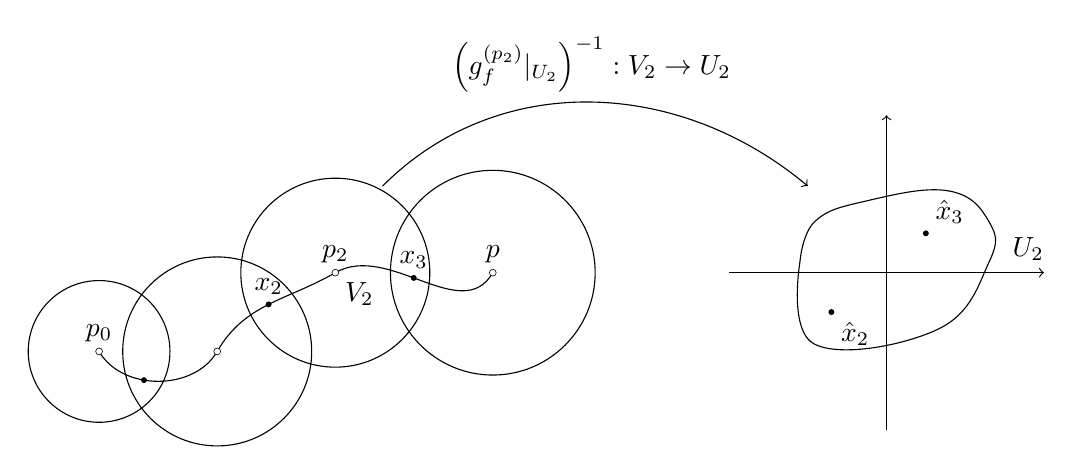
\begin{tikzpicture}
\def\px{0cm}
\def\py{0cm}
\def\qx{5cm}
\def\qy{1cm}
\def\sx{1.5cm}
\def\sy{0cm}
\def\tx{3cm}
\def\ty{1cm}
\draw[fill] (\px,\py) circle (.04) node[above] {\(p_0\)};
\draw[fill] (\sx,\sy) circle (.04);
\draw[fill] (\tx,\ty) circle (.04) node[above] {\(p_2\)};
\draw[fill] (\qx,\qy) circle (.04) node[above] {\(p\)};

\draw (\px,\py) to[out = -60, in = -120] coordinate[pos = .4] (x1) (\sx,\sy) to[out = 60, in = -150]coordinate[pos = .5] (x2) (\tx,\ty) to[out = 30, in = -120]coordinate[pos = .45] (x3) (\qx,\qy);

\draw[fill] (x1) circle (.03);
\draw[fill] (x2) circle (.03) node[above] {\(x_2\)};
\draw[fill] (x3) circle (.03) node[above] {\(x_3\)};
%\draw[fill, color = white] (x1) circle (.03);
%\draw[fill, color = white] (x2) circle (.03);
%\draw[fill, color = white] (x3) circle (.03);

\draw (\px,\py) circle (.9);
\draw (\sx,\sy) circle (1.2);
\draw (\tx,\ty) circle (1.2);
\draw (\qx,\qy) circle (1.3);
\node[anchor = north west] at (\tx,\ty) {\(V_2\)};

\draw[fill, color = white] (\px,\py) circle (.03);
\draw[fill, color = white] (\sx,\sy) circle (.03);
\draw[fill, color = white] (\tx,\ty) circle (.03);
\draw[fill, color = white] (\qx,\qy) circle (.03);

\draw[-to] ({\tx + .6cm},{\ty + 1.1cm}) to[out = 45, in = 140]node[pos = .5, anchor = south] {\(\left(g_f^{({p_2})}|_{U_2}\right)^{-1}:V_2\to U_2\)} ({\tx + 6cm},{\ty + 1.1cm});

\begin{scope}[xshift = {\tx + 7cm}, yshift = {\ty}]
\draw[->] (0,0) -- ++ (0,-2) -- ++ (0,4);
\draw[->] (0,0) -- ++ (-2,0) -- ++ (4,0);
\draw plot[smooth, tension=.7] coordinates {(-1.1,0.13) (-.91,.65) (-.26,.91) (.78,1.04) (1.3,.65) (1.3,0.13) (.65,-.72) (-.91,-.91) (-1.1,0.13)};
\node at (1.8,.3) {\(U_2\)};
\draw[fill] (.5,.5) circle (.03) node[anchor = south west] {\(\hat{x}_3\)};
\draw[fill] (-.7,-.5) circle (.03) node[anchor = north west] {\(\hat{x}_2\)};
%\draw[fill, white] (.5,.5) circle (.03);
%\draw[fill, white] (-.7,-.5) circle (.03);
\end{scope}
\end{tikzpicture}
\end{document}